% !TEX program = xelatex
% ============================================================================
%  POSN Computer Qualification — Exponential & Logarithmic Functions
%  Topic: ฟังก์ชันเอกซ์โพเนนเชียลและลอการิทึม
% ============================================================================

\documentclass[11pt, aspectratio=169]{beamer}
% ============================================================================
%  POSN Computer Qualification — Shared Beamer Preamble
%  Used by all topic slide decks. Compile with XeLaTeX.
% ============================================================================

% ---------- Thai language & font ----------
\usepackage{iftex}
\usepackage{fontspec}

% XeTeX-specific: enable Thai line breaking
\ifXeTeX
  \XeTeXlinebreaklocale{th}
\fi
% Noto Sans Thai — body text (clean modern sans-serif, handles all Thai)
\setmainfont{Noto Sans Thai}[
  UprightFont = Noto Sans Thai Light,
  BoldFont    = Noto Sans Thai Medium,
  Scale       = 0.9
]
\setsansfont{Noto Sans Thai}[
  UprightFont = Noto Sans Thai Light,
  BoldFont    = Noto Sans Thai Medium,
  Scale       = 0.9
]

% Noto Sans Thai — clean modern sans-serif for structural elements
\newfontfamily\headingfont{Noto Sans Thai}[
  UprightFont = Noto Sans Thai Medium,
  BoldFont    = Noto Sans Thai Bold,
  Scale       = 0.9
]

% --- Heading font for structural elements ---
\setbeamerfont{title}{family=\headingfont, series=\bfseries, size=\huge}
\setbeamerfont{subtitle}{family=\headingfont, series=\mdseries}
\setbeamerfont{author}{family=\headingfont, series=\mdseries}

% --- Custom Title Page ---
\defbeamertemplate{title page}{custom}[1][]{%
  \centering
  \vspace*{2cm}
  % Title — in white
  {\usebeamerfont{title}\color{white}\inserttitle\par}
  \vspace{0.6cm}
  % Subtitle — in white
  {\usebeamerfont{subtitle}\color{white}\insertsubtitle\par}
  \vspace{2.5cm}
  % Author — blue filled rounded box, white text
  \begin{center}
    \begin{tcolorbox}[arc=3mm, colback=boxBlue, colframe=boxBlue!80,
                      width=0.42\textwidth, halign=center,
                      left=1.5em, right=1.5em, top=0.8em, bottom=0.8em,
                      boxrule=1.5pt, coltext=white]
      \usebeamerfont{author}\insertauthor
    \end{tcolorbox}
  \end{center}
}
\setbeamertemplate{title page}[custom]
\setbeamerfont{frametitle}{family=\headingfont, series=\bfseries}
\setbeamerfont{section in toc}{family=\headingfont}
\setbeamerfont{page number in head/foot}{family=\headingfont}
\setbeamerfont{section title}{family=\headingfont, series=\bfseries}
\setbeamerfont{subsection title}{family=\headingfont}

% Monospace font (for code/verbatim)
\setmonofont{Latin Modern Mono}[Scale=0.9]

% ---------- Math ----------
\usepackage{amsmath, amssymb}

% ---------- Graphics ----------
\usepackage{graphicx}
\usepackage{tikz}

% ---------- String parsing (for section headers) ----------
\usepackage{xstring}

% ---------- Colored boxes ----------
\usepackage[skins, breakable, xparse]{tcolorbox}
% Note: we do NOT load the 'most' option — it predefines example/solution environments
% that would conflict with our custom boxes.

% --- Color definitions ---
\definecolor{boxBlue}{RGB}{41, 128, 185}
\definecolor{boxGreen}{RGB}{39, 174, 96}
\definecolor{boxOrange}{RGB}{230, 126, 34}
\definecolor{boxPurple}{RGB}{142, 68, 173}
\definecolor{boxBlueBg}{RGB}{235, 245, 255}
\definecolor{boxGreenBg}{RGB}{235, 255, 240}
\definecolor{boxOrangeBg}{RGB}{255, 245, 235}
\definecolor{boxPurpleBg}{RGB}{248, 240, 255}

% --- Explanation box (blue) — for definitions, concepts, notes ---
\newtcolorbox{explanation}[1][]{
  enhanced,
  breakable,
  arc         = 2mm,
  colback     = boxBlueBg,
  colframe    = boxBlue!50,
  title       = #1,
  fonttitle   = \bfseries\color{white},
  coltitle    = white,
  colbacktitle= boxBlue,
  attach boxed title to top left = {yshift=-2mm, xshift=2mm},
  boxed title style = {arc=2mm, size=small},
  before skip = 8pt,
  after skip  = 8pt
}

% --- Example box (green) — for worked examples ---
\newtcolorbox{exambox}[1][]{
  enhanced,
  breakable,
  arc         = 2mm,
  colback     = boxGreenBg,
  colframe    = boxGreen!50,
  title       = #1,
  fonttitle   = \bfseries\color{white},
  coltitle    = white,
  colbacktitle= boxGreen,
  attach boxed title to top left = {yshift=-2mm, xshift=2mm},
  boxed title style = {arc=2mm, size=small},
  before skip = 8pt,
  after skip  = 8pt
}

% --- Solution box (orange) — for solutions and answers ---
\newtcolorbox{solbox}[1][]{
  enhanced,
  breakable,
  arc         = 2mm,
  colback     = boxOrangeBg,
  colframe    = boxOrange!50,
  title       = #1,
  fonttitle   = \bfseries\color{white},
  coltitle    = white,
  colbacktitle= boxOrange,
  attach boxed title to top left = {yshift=-2mm, xshift=2mm},
  boxed title style = {arc=2mm, size=small},
  before skip = 8pt,
  after skip  = 8pt
}

% --- Intuition box (purple) — for plain-language explanations, analogies ---
\newtcolorbox{intuition}[1][]{
  enhanced,
  breakable,
  arc         = 2mm,
  colback     = boxPurpleBg,
  colframe    = boxPurple!50,
  title       = #1,
  fonttitle   = \bfseries\color{white},
  coltitle    = white,
  colbacktitle= boxPurple,
  attach boxed title to top left = {yshift=-2mm, xshift=2mm},
  boxed title style = {arc=2mm, size=small},
  before skip = 8pt,
  after skip  = 8pt
}

% ---------- Beamer theme ----------
\usetheme{Madrid}
\usecolortheme{default}

% --- Custom beamer colors (blue accent matching explanation boxes) ---
\setbeamercolor{structure}{fg=boxBlue}
\setbeamercolor{palette primary}{fg=white, bg=boxBlue}
\setbeamercolor{palette secondary}{fg=white, bg=boxBlue!80}
\setbeamercolor{palette tertiary}{fg=white, bg=boxBlue!60}
\setbeamercolor{block title}{fg=white, bg=boxBlue}
\setbeamercolor{block body}{fg=black, bg=boxBlueBg}

% Remove navigation symbols for clean look
\setbeamertemplate{navigation symbols}{}

% Note: Frame title prefix removed — \addtobeamertemplate conflicts with beamer internals

% --- Outline (Table of Contents) styling ---
\setbeamerfont{section in toc}{family=\headingfont, series=\mdseries}
\setbeamerfont{subsection in toc}{family=\headingfont, series=\mdseries}
\setbeamertemplate{section in toc}{%
  \leavevmode\leftskip=1.5em
  \textcolor{boxBlue}{\textbf{\large\inserttocsectionnumber.}}%
  \quad\inserttocsection\par
  \vspace{0.2em}
}
\setbeamertemplate{subsection in toc}{%
  \leavevmode\leftskip=4em
  \textcolor{boxBlue!60}{\small$\bullet$}%
  \quad\inserttocsubsection\par
  \vspace{0.1em}
}

% Section header slides — Thai in white, English in smaller light blue below
\AtBeginSection{
  \begin{frame}[plain]{}
    \vspace*{2cm}
    \begin{beamercolorbox}[sep=12pt, center, rounded=true, shadow=true]{palette primary}
      \IfSubStr{\secname}{(}{%
        \StrBefore{\secname}{(}[\sectionthai]%
        \StrBetween[1,1]{\secname}{(}{)}[\sectioneng]%
        \begin{tabular}{@{}c@{}}
          {\usebeamerfont{title}\sectionthai} \\[0.2em]
          {\usebeamerfont{subtitle}\color{boxBlue!60}\sectioneng}
        \end{tabular}%
      }{%
        {\usebeamerfont{title}\secname\par}%
      }
    \end{beamercolorbox}
    \vfill
  \end{frame}
}

% Subsection header slides — smaller, centered
\AtBeginSubsection{
  \begin{frame}[plain]{}
    \vfill
    \centering
    {\usebeamerfont{section title}\insertsubsectionhead\par}
    \vfill
  \end{frame}
}

% Minimal footer: page number only, right-aligned
\setbeamertemplate{footline}{
  \hfill\usebeamerfont{page number in head/foot}\insertframenumber{} / \inserttotalframenumber\hspace*{1em}\vspace*{0.5ex}
}

% ---------- Spacing & readability ----------
\linespread{1.2}

% ---------- Useful commands ----------

% Highlight important text in blue
\newcommand{\highlight}[1]{\textcolor{boxBlue}{\textbf{#1}}}

% Math set notation helpers
\newcommand{\R}{\mathbb{R}}
\newcommand{\N}{\mathbb{N}}
\newcommand{\Z}{\mathbb{Z}}
\newcommand{\Q}{\mathbb{Q}}

% ============================================================================
%  End of preamble
% ============================================================================


\title[เอกซ์โพเนนเชียลและลอการิทึม]{\textcolor{white}{ฟังก์ชันเอกซ์โพเนนเชียลและลอการิทึม} \\ \textcolor{boxBlue!60}{(Exponential \& Logarithmic Functions)}}
\subtitle{ฟังก์ชันเอกซ์โพเนนเชียล • ฟังก์ชันลอการิทึม • สมบัติของลอการิทึม • การแก้สมการ }
\author[None W. (Yuan)]{None W. (Yuan)}
\date{}

\begin{document}

\begin{frame}[plain]\titlepage\end{frame}
\begin{frame}{สารบัญ (Outline)}\tableofcontents\end{frame}

\begin{frame}{ก่อนเรียน (Prerequisites)}
  \begin{explanation}[สิ่งที่ควรรู้ก่อนเรียน]
    \begin{itemize}
      \item \textbf{เลขยกกำลัง} — $a^m \cdot a^n = a^{m+n}$, $(a^m)^n = a^{mn}$, $a^{-n} = \frac{1}{a^n}$
      \item \textbf{ฟังก์ชัน} — โดเมน, เรนจ์, ฟังก์ชันผกผัน
    \end{itemize}
  \end{explanation}

  \begin{intuition}[แนวคิดสำคัญ]
    \textbf{Exponential} ($a^x$) กับ \textbf{Logarithm} ($\log_a x$) เป็น \highlight{ฟังก์ชันผกผัน}ซึ่งกันและกัน
  \end{intuition}
\end{frame}

% ===========================================================================
%  SECTION 1: ฟังก์ชันเอกซ์โพเนนเชียล
% ===========================================================================
\section{ฟังก์ชันเอกซ์โพเนนเชียล}

\begin{frame}{ฟังก์ชันเอกซ์โพเนนเชียล}
  \begin{explanation}[นิยาม]
    $f(x) = a^x$ \quad โดย $a > 0$, $a \neq 1$
  \end{explanation}

  \begin{columns}[T]
    \column{0.5\textwidth}
      \centering
      \textbf{$a > 1$: ฟังก์ชันเพิ่ม}
      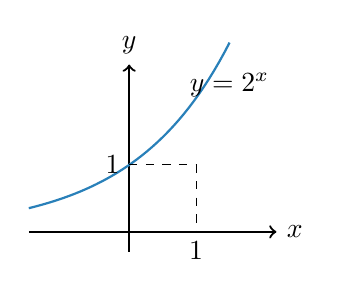
\begin{tikzpicture}[scale=0.85]
        \draw[->,thick] (-1.5,0) -- (2.2,0) node[right] {$x$};
        \draw[->,thick] (0,-0.3) -- (0,2.5) node[above] {$y$};
        \draw[boxBlue, thick, domain=-1.5:1.5, samples=40]
          plot (\x, {1.0*2.0^\x});
        \draw[dashed] (0,1) node[left] {$1$} -- (1,1) -- (1,0) node[below] {$1$};
        \node at (1.5,2.2) {$y = 2^x$};
      \end{tikzpicture}
      \begin{itemize}
        \item โดเมน $= \R$, เรนจ์ $= (0, \infty)$
        \item ผ่าน $(0,1)$ เสมอ, แกน $x$ เป็นเส้นกำกับ
      \end{itemize}

    \column{0.5\textwidth}
      \centering
      \textbf{$0 < a < 1$: ฟังก์ชันลด}
      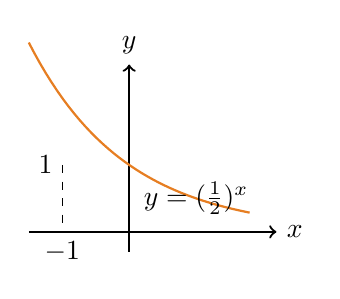
\begin{tikzpicture}[scale=0.85]
        \draw[->,thick] (-1.5,0) -- (2.2,0) node[right] {$x$};
        \draw[->,thick] (0,-0.3) -- (0,2.5) node[above] {$y$};
        \draw[boxOrange, thick, domain=-1.5:1.8, samples=40]
          plot (\x, {1.0*0.5^\x});
        \draw[dashed] (-1,1) node[left] {$1$} -- (-1,0) node[below] {$-1$};
        \node at (1.0,0.5) {$y = (\frac{1}{2})^x$};
      \end{tikzpicture}
      \begin{itemize}
        \item โดเมน $= \R$, เรนจ์ $= (0, \infty)$
        \item ผ่าน $(0,1)$ เสมอ, แกน $x$ เป็นเส้นกำกับ
      \end{itemize}
  \end{columns}
\end{frame}

\begin{frame}{สมบัติของเลขยกกำลัง}
  \begin{explanation}[สูตรพื้นฐาน]
    \begin{columns}[T]
      \column{0.5\textwidth}
        \begin{itemize}
          \item $a^m \cdot a^n = a^{m+n}$
          \item $\dfrac{a^m}{a^n} = a^{m-n}$
          \item $(a^m)^n = a^{mn}$
        \end{itemize}
      \column{0.5\textwidth}
        \begin{itemize}
          \item $a^0 = 1$ \quad ($a \neq 0$)
          \item $a^{-n} = \dfrac{1}{a^n}$
          \item $a^{1/n} = \sqrt[n]{a}$
        \end{itemize}
    \end{columns}
  \end{explanation}

  \begin{exambox}[ตัวอย่าง]
    $2^3 \cdot 2^4 = 2^{7} = 128$ \qquad
    $(3^2)^3 = 3^{6} = 729$ \qquad
    $8^{1/3} = \sqrt[3]{8} = 2$
  \end{exambox}
\end{frame}

% ===========================================================================
%  SECTION 2: ฟังก์ชันลอการิทึม
% ===========================================================================
\section{ฟังก์ชันลอการิทึม}

\begin{frame}{ลอการิทึมคืออะไร?}
  \begin{explanation}[นิยาม]
    $\log_a x = y$ \quad ก็ต่อเมื่อ \quad $a^y = x$ \qquad ($a > 0$, $a \neq 1$, $x > 0$)

    \highlight{ลอการิทึมคือเลขชี้กำลัง!} $\log_a x$ คือเลขชี้กำลังที่ยก $a$ แล้วได้ $x$
  \end{explanation}

  \begin{columns}[T]
    \column{0.5\textwidth}
      \begin{exambox}[ตัวอย่าง]
        $\log_2 8 = 3$ \quad $(2^3 = 8)$

        $\log_5 25 = 2$ \quad $(5^2 = 25)$

        $\log_{10} 1000 = 3$ \quad $(10^3 = 1000)$
      \end{exambox}
    \column{0.5\textwidth}
      \begin{exambox}[ค่าพิเศษ]
        $\log_a 1 = 0$ \quad $\log_a a = 1$

        $\log_a a^x = x$ \quad $a^{\log_a x} = x$
      \end{exambox}
  \end{columns}
\end{frame}

\begin{frame}{กราฟของฟังก์ชันลอการิทึม}
  \begin{columns}[T]
    \column{0.5\textwidth}
      \centering
      \textbf{$a > 1$: ฟังก์ชันเพิ่ม}
      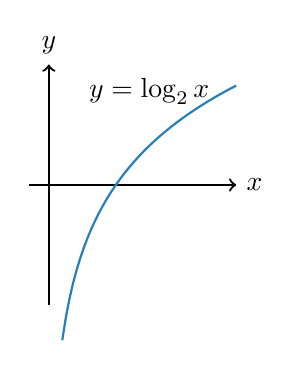
\begin{tikzpicture}[scale=0.85]
        \draw[->,thick] (-0.3,0) -- (2.8,0) node[right] {$x$};
        \draw[->,thick] (0,-1.8) -- (0,1.8) node[above] {$y$};
        \draw[boxBlue, thick, domain=0.2:2.8, samples=50]
          plot (\x, {ln(\x)/ln(2)});
        % \draw[dashed] (1,0) node[below] {$1$} -- (1,1) node[left] {$1$};
        \node at (1.5,1.4) {$y = \log_2 x$};
      \end{tikzpicture}
      \begin{itemize}
        \item โดเมน $= (0, \infty)$, เรนจ์ $= \R$
        \item ผ่าน $(1,0)$ เสมอ
      \end{itemize}

    \column{0.5\textwidth}
      \centering
      \textbf{$0 < a < 1$: ฟังก์ชันลด}
      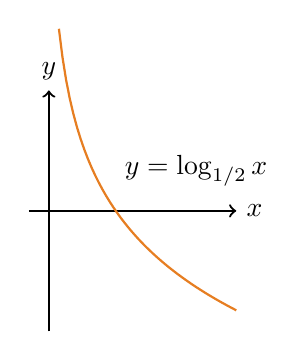
\begin{tikzpicture}[scale=0.85]
        \draw[->,thick] (-0.3,0) -- (2.8,0) node[right] {$x$};
        \draw[->,thick] (0,-1.8) -- (0,1.8) node[above] {$y$};
        \draw[boxOrange, thick, domain=0.15:2.8, samples=50]
          plot (\x, {ln(\x)/ln(0.5)});
        % \draw[dashed] (1,0) node[above] {$1$} -- (2,1) -- (2,0) node[below] {$2$};
        \node at (2.2,0.6) {$y = \log_{1/2} x$};
      \end{tikzpicture}
      \begin{itemize}
        \item โดเมน $= (0, \infty)$, เรนจ์ $= \R$
        \item ผ่าน $(1,0)$ เสมอ
      \end{itemize}
  \end{columns}
\end{frame}

% ===========================================================================
%  SECTION 3: สมบัติของลอการิทึม
% ===========================================================================
\section{สมบัติของลอการิทึม}

\begin{frame}{สมบัติของลอการิทึม}
  \begin{explanation}[สูตรพื้นฐาน]
    $\log_a (MN) = \log_a M + \log_a N$ \qquad
    $\log_a \left(\dfrac{M}{N}\right) = \log_a M - \log_a N$

    $\log_a M^p = p \log_a M$ \qquad
    $\log_a b = \dfrac{\log_c b}{\log_c a}$ \quad (เปลี่ยนฐาน)
  \end{explanation}

  \begin{exambox}[ตัวอย่าง]
    $\log_2 (8 \times 4) = \log_2 8 + \log_2 4 = 3 + 2 = 5$ \quad
    $\log_3 3^5 = 5 \log_3 3 = 5$

    $\log_8 2 = \dfrac{\log_2 2}{\log_2 8} = \dfrac{1}{3}$
  \end{exambox}
\end{frame}

\begin{frame}{ความสัมพันธ์ระหว่าง exp และ log}
  \begin{explanation}[ฟังก์ชันผกผัน]
    $f(x) = a^x$ และ $g(x) = \log_a x$ เป็น \highlight{ฟังก์ชันผกผัน}ซึ่งกันและกัน
    (กราฟสะท้อนกันโดยมี $y = x$ เป็นแกนสะท้อน)
  \end{explanation}

  \begin{center}
    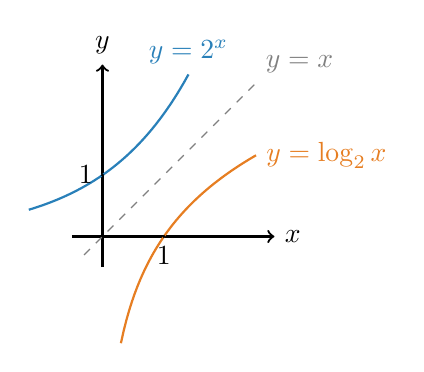
\begin{tikzpicture}[scale=0.78]
      \draw[->,thick] (-0.5,0) -- (2.8,0) node[right] {$x$};
      \draw[->,thick] (0,-0.5) -- (0,2.8) node[above] {$y$};
      \draw[gray, dashed] (-0.3,-0.3) -- (2.5,2.5) node[above right] {$y=x$};
      \draw[boxBlue, thick, domain=-1.2:1.4, samples=40]
        plot (\x, {1.0*2.0^\x}) node[above] {$y=2^x$};
      \draw[boxOrange, thick, domain=0.3:2.5, samples=50]
        plot (\x, {ln(\x)/ln(2)}) node[right] {$y=\log_2 x$};
      \fill (0,1) circle (0.8pt) node[left] {$1$};
      \fill (1,0) circle (0.8pt) node[below] {$1$};
    \end{tikzpicture}
  \end{center}
\end{frame}

% ===========================================================================
%  SECTION 4: การแก้สมการ
% ===========================================================================
\section{การแก้สมการ}

\begin{frame}{การแก้สมการ}
  \begin{exambox}[ตัวอย่าง]
    \textbf{สมการเอกซ์โพเนนเชียล:}

    $2^{x+1}=16 \;\rightarrow\; x=3$ \qquad
    $3^{2x}=27 \;\rightarrow\; x=\frac{3}{2}$ \qquad
    $5^x=7 \;\rightarrow\; x=\log_5 7$

    \medskip
    \textbf{สมการลอการิทึม:}

    $\log_2(x+1)=3 \;\rightarrow\; x=7$ \qquad
    $\log_3 x + \log_3(x-2)=1 \;\rightarrow\; \log_3[x(x-2)]=1 \;\rightarrow\; x=3$
  \end{exambox}
\end{frame}

% ===========================================================================
%  SUMMARY
% ===========================================================================
\section{สรุป}

\begin{frame}{สรุปเนื้อหา}
  \begin{explanation}[สิ่งที่ได้เรียนรู้]
    \begin{columns}[T]
      \column{0.5\textwidth}
        \textbf{Exponential $f(x) = a^x$}
        \begin{itemize}
          \item $a > 1$: เพิ่ม, $0 < a < 1$: ลด
          \item โดเมน $= \R$, เรนจ์ $= (0, \infty)$
          \item ผ่าน $(0,1)$, แกน $x$ เป็นเส้นกำกับ
          \item $a^m a^n = a^{m+n}$, $(a^m)^n = a^{mn}$
        \end{itemize}
      \column{0.5\textwidth}
        \textbf{Logarithm $\log_a x$}
        \begin{itemize}
          \item $\log_a x = y \iff a^y = x$
          \item โดเมน $= (0, \infty)$, เรนจ์ $= \R$
          \item ผ่าน $(1,0)$, แกน $y$ เป็นเส้นกำกับ
          \item $\log(MN) = \log M + \log N$
          \item เปลี่ยนฐาน: $\log_a b = \frac{\log_c b}{\log_c a}$
        \end{itemize}
    \end{columns}

    \medskip
    \begin{center}
      \highlight{Exponential และ Logarithm เป็นฟังก์ชันผกผันซึ่งกันและกัน}
    \end{center}
  \end{explanation}
  \begin{center}
    \large เอกสารนี้เป็นส่วนหนึ่งของเนื้อหาเตรียมสอบ \textbf{สอวน. คอมพิวเตอร์}
  \end{center}
\end{frame}

\end{document}
